\documentclass[fleqn]{extarticle}
\usepackage{amsmath, amssymb}
\usepackage[russian]{babel}
\usepackage{graphicx}

\textwidth 18cm
\textheight 25cm
\oddsidemargin -1cm
\evensidemargin -1cm
\topmargin -3cm
\pdfpageheight 297mm

\newcommand{\pares}[1]{ \left( #1 \right) }

\title{Углы Тейта-Брайана и Эйлера. Лекционный материал.\\Аналитическая геометрия}
\author{AriosJentu}
\date{}

\begin{document}

	\maketitle

	Для достижения всех возможных ориентаций объекта в $R^3$ необходимо учитывать три степени свободы. 
	Например, в управлении воздушным судном их обычно называют креном, тангажем и рысканьем. 
	Крен (Roll) -- это вращение вдоль оси вперед-назад. 
	Тангаж (Pitch) -- это вращение вдоль оси из стороны в сторону, что соответствует плоскости, направленной вверх или вниз.
	Рысканье (Yaw) -- это вращение вокруг вертикальной оси. Все это необходимо для правильного функционирования самолета.

	\section{Углы Тейта-Брайана}

	Один из способов добиться всех возможных ориентаций -- разрешить повороты по каждой из основных осей, 
	а затем объединить эти повороты, чтобы сориентировать объект. 
	Безусловно, таким образом можно добиться любой ориентации.

	Матрица поворота вокруг оси $x$ на угол $\alpha$ имеет вид:
	\[ R_x = \begin{pmatrix} 1 & 0 & 0 \\ 0 & \cos{\alpha} & -\sin{\alpha} \\ 0 & \sin{\alpha} & \cos{\alpha} \end{pmatrix}; \]
	аналогично, вокруг оси $y$ на угол $\beta$ и вокруг оси $z$ на угол $\gamma$, соответственно:
	\[ R_y = \begin{pmatrix} \cos{\beta} & 0 & \sin{\beta} \\ 0 & 1 & 0 \\ -\sin{\beta} & 0 & \cos{\beta} \end{pmatrix}; \quad R_z = \begin{pmatrix} \cos{\gamma} & -\sin{\gamma} & 0 \\ \sin{\gamma} & \cos{\gamma} & 0 \\ 0 & 0 & 1 \end{pmatrix}; \] 

	Для каждого из них направление вращения соответствует правилу правой руки, 
	при этом большой палец указывает в положительном направлении каждой оси.
	Чтобы добиться любой ориентации нашего объекта, нам, вероятно, понадобятся все три этих поворота. 

	Но как их совместить?
	Обычно выбирается порядок, а затем результат может быть использован для получения любой желаемой ориентации.
	Если выбрать вращения, например изначально в оси $z$, затем $y$, и затем $x$, то поворот определим следующим преобразованием:
	\[ R_{xyz}(\alpha, \beta, \gamma) = R_x(\alpha) \cdot R_y(\beta) \cdot R_z(\gamma). \]

	К примеру, предположим самолет, летящий по положительному направлению оси $x$, и нам нужно его развернуть в сторону движения вдоль оси $y$. 
	Положим, что он направлен вектором с координатами $(1, 0, 0)$, тогда его требуется повернуть на $\frac{\pi}{2}$ вокруг оси $z$. Углы тогда будут $\left(0, 0, \frac{\pi}{2} \right)$. 
	Матрица поворота тогда отвечает за блок управления самолётом:
	\[ R_x = I, ~ R_y = I, ~ R_z = \begin{pmatrix} 0 & -1 & 0 \\ 1 & 0 & 0 \\ 0 & 0 & 1 \end{pmatrix}. \]
	Тогда новое направление движения будет получено путем умножения матрицы поворота на исходный вектор:
	\[ \begin{pmatrix} 0 & -1 & 0 \\ 1 & 0 & 0 \\ 0 & 0 & 1 \end{pmatrix} \cdot \begin{pmatrix} 1 \\ 0 \\ 0 \end{pmatrix} = \begin{pmatrix} 0 \\ 1 \\ 0 \end{pmatrix}, \]
	что теперь и указывает вдоль положительного направления по оси $y$.

	Рассмотрим теперь случай поворота на углы $\left(\alpha, \frac{\pi}{2}, \gamma \right)$ соответственно:
	\[ R_y = \begin{pmatrix} 0 & 0 & 1 \\ 0 & 1 & 0 \\ -1 & 0 & 0 \end{pmatrix}. \]
	Перемножая $R_x, R_y, R_z$, получим матрицу:
	\[ R_x \cdot R_y \cdot R_z = \begin{pmatrix} 
		0 & 0 & 1 \\ \sin{\alpha} & \cos{\alpha} & 0 \\ -\cos{\alpha} & \sin{\alpha} & 0 
	\end{pmatrix} \cdot \begin{pmatrix} 
		\cos{\gamma} & -\sin{\gamma} & 0 \\ \sin{\gamma} & \cos{\gamma} & 0 \\ 0 & 0 & 1 
	\end{pmatrix} \]
	\[ R_{xyz} = \begin{pmatrix} 
		0 & 0 & 1 \\ \sin(\alpha + \gamma) & \cos(\alpha + \gamma) & 0 \\ -\cos(\alpha + \gamma) & \sin(\alpha + \gamma) & 0
	\end{pmatrix} \]

	В этот момент наш блок управления утратил некоторые функциональные возможности, 
	потому что изменение двух входных параметров $\alpha$ и $\gamma$ оказывает одинаковое влияние на выходную матрицу. 
	Более того, если мы увеличим $\alpha$ и уменьшим $\gamma$ на одинаковую величину, выходная матрица не изменится.

	Результат может становиться еще хуже. Из этой конкретной настройки углов
	$\left(\alpha, \beta \gamma \right) = \left(0, \frac{\pi}{2}, 0 \right)$ 
	можно изменить любую комбинацию $\alpha, \beta$ и $\gamma$ таким образом, 
	что это приведет к небольшому вращению вокруг оси $z$.

	Положим объект с двумя ключевыми точками -- $P = (0, 1, 0)$ и $Q = (-1, 0, 0)$. Стоит обратить внимание, что 
	\[ R_{x, y, z}\left(0, \frac{\pi}{2}, 0 \right) \cdot \begin{pmatrix} 0 \\ 1 \\ 0 \end{pmatrix} = \begin{pmatrix} 0 \\ 1 \\ 0 \end{pmatrix} = P' \] 
	Точка $P'$ находится в плоскости $Oxy$;
	\[ R_{x, y, z}\left(0, \frac{\pi}{2}, 0 \right) \cdot \begin{pmatrix} -1 \\ 0 \\ 0 \end{pmatrix} = \begin{pmatrix} 0 \\ 0 \\ 1 \end{pmatrix} = Q' \]
	В свою очередь точка $Q'$ теперь лежит на оси $z$.

	Предположим, что мы хотим внести изменения в углы ввода блока управления, 
	чтобы повернуть результирующую точку $P'$ вокруг оси $z$. Это означает, что $P'$ должна двигаться 
	(в частности, координата $y$ должна уменьшаться, в то время как $x$ может увеличиваться или уменьшаться), 
	в то время как $Q'$ должна оставаться на месте.

	Рассмотрим, что произойдет в момент, если мы добавим небольшого возмущения к $\alpha, \beta$ и $\gamma$ в виде $a \approx 0, ~ b \approx 0, ~ c \approx 0$:
	\[ R_{x, y, z}\left(a, \frac{\pi}{2} + b, c \right) \cdot \begin{pmatrix} 0 \\ 1 \\ 0 \end{pmatrix} = \begin{pmatrix} \sin{b}\sin{c} \\ \cos{a}\cos{c} - \sin{a} \cos{b} \sin{c} \\ \sin{a} \cos{c} + \cos{a} \cos{b} \sin{c} \end{pmatrix} = P'' \]
	и
	\[ R_{x, y, z}\left(a, \frac{\pi}{2} + b, c \right) \cdot \begin{pmatrix} -1 \\ 0 \\ 0 \end{pmatrix} = \begin{pmatrix} \sin{b} \cos{c} \\ -\cos{a}\sin{c} - \sin{a} \cos{b} \cos{c} \\ \cos{a} \cos{b} \cos{c} - \sin{a} \sin{c} \end{pmatrix} = Q'' \]

	Наше пожелание состоит в том, чтобы выбрать $a, b, c$ такими, чтобы точка $Q'' = Q'$, и при этом точка $P''$ представляла из себя точку $P'$, претерпевающую небольшой поворот вокруг оси $z$.

	Чтобы сохранить $Q'' = Q' = (0, 0, 1)$, нам нужно, чтобы первая строка $\sin{b} \cos{c}$ оставалась равной $0$. 
	Для этого необходимо, чтобы $b$ оставалась равной нулю. При $c \approx 0$, известно, что $\cos{c} \approx 1$.

	Однако, если $b$ остается равным $0$, то первая строка $P''$ -- $\sin{b} \sin{c}$ также остается равной $0$, 
	а это означает, что мы не можем изменить координату $x$ точки $P'$. Соответственно это не позволит нам провести 
	вращение, так как ось $x$ теперь заблокирована. Такая ситуация называется блокировкой оси, и может встречаться повсеместно 
	в случае углов Тейта-Брауна, как и в углах Эйлера, о которых речь пойдет дальше.

	\begin{figure}[h]
		\centering
		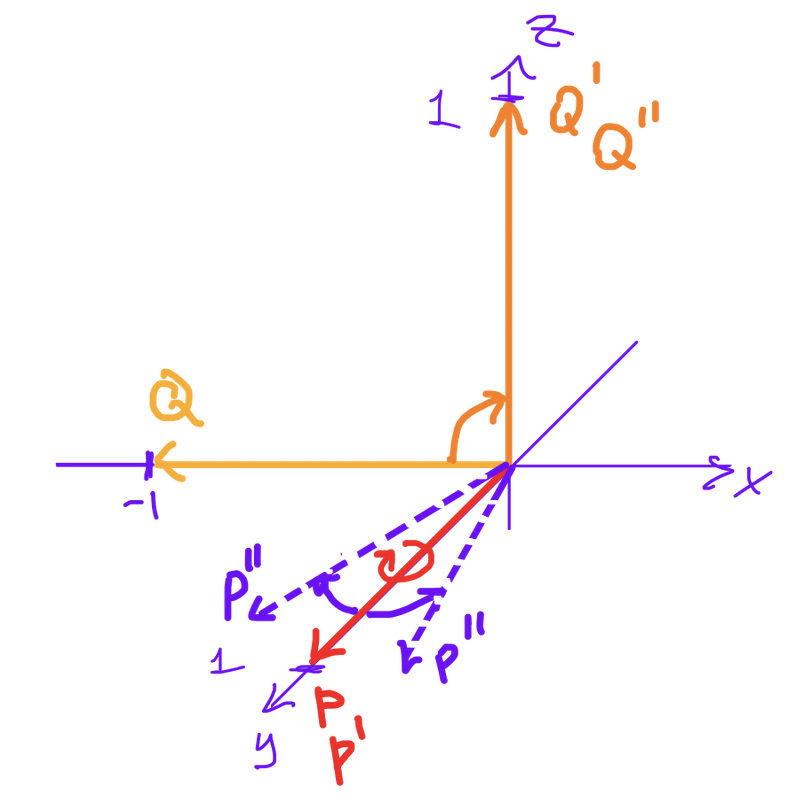
\includegraphics[width=7cm]{pictures/bryan.png}
		\caption{Углы Тейта-Брайана}
	\end{figure}

	\pagebreak
	\section{Углы Эйлера}

	Более классическим вариантом организации поворотов объектов в трехмерном пространстве является алгоритм поворота Эйлера, 
	и включает в себя рассмотрение двух ортогональных систем координат с общим центром -- исходная 
	подвижная ($Oxyz$), и результирующая неподвижная ($Ox'y'z'$). В классическом варианте поворот 
	состоит из трех последовательных этапов:
	\begin{enumerate}
		\item Переход в систему $O\tilde{x}\tilde{y}z$: поворот на угол $\alpha$ (угол \textit{прецессии}) 
			вокруг оси $Z$, после чего ось $X$ окажется в плоскости $Ox'y'$. Такое совмещение произойдет по 
			линии узлов (линия $N$). пересечения плоскостей $Oxy$ и $Ox'y'$. 

		\item Переход в систему $O\tilde{x}\bar{y}z'$: поворот на угол $\beta$ (угол \textit{нутации}) вокруг новой 
			оси $\tilde{X}$, после которого оси $Z$ и $Z'$ совпадут. При этом ось $Y'$ окажется в плоскости $Ox'y'$.

		\item Переход в систему $Ox'y'z'$: поворот на угол $\gamma$ (угол \textit{собственного вращения}) вокруг 
			оси $Z'$, после которого оси $\tilde{X}$ и $\bar{y}$ совпадут соответственно с осями $X'$ и $Y'$. 
	\end{enumerate}

	Результирующая матрица преобразования поворота собирается из матриц поворота следующим образом:
	\[ R_{zxz}(\alpha, \beta, \gamma) = R_z(\gamma) \cdot R_x(\beta) \cdot R_z(\alpha). \]

	\begin{figure}[h]
		\centering
		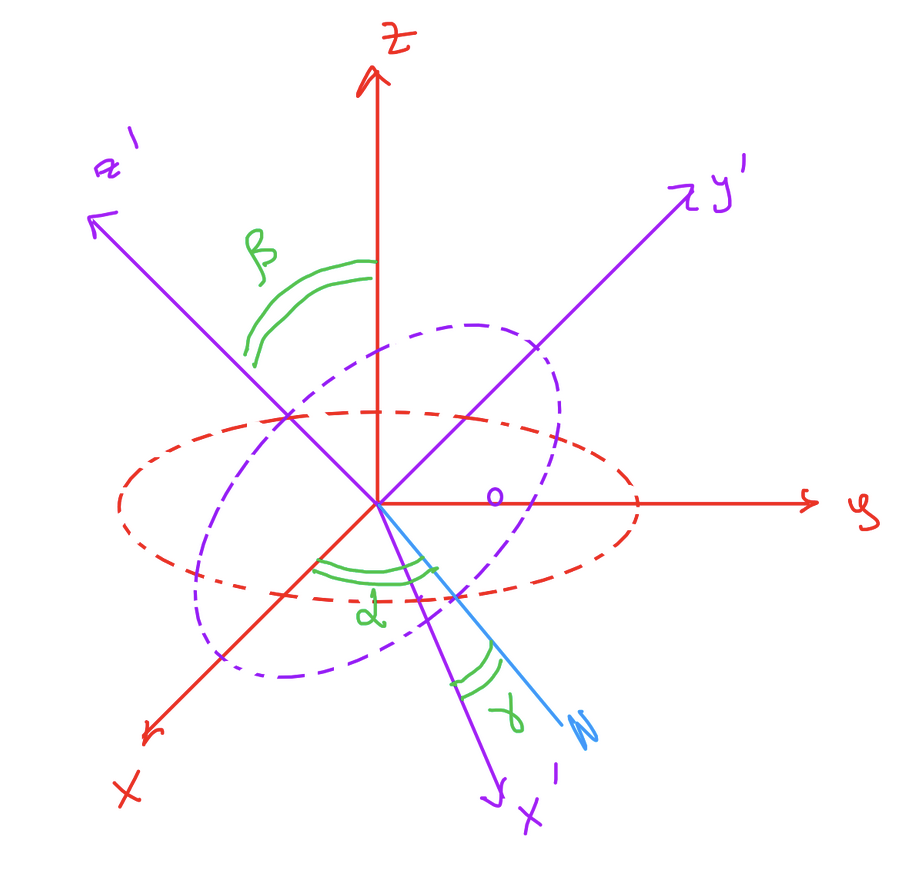
\includegraphics[width=7cm]{pictures/euler.png}
		\caption{Углы Эйлера}
	\end{figure}


\end{document}